\documentclass{mirea}

\institution{Институт искусственного интеллекта}
\faculty    {Кафедра общей информатики}
\worktype   {ОТЧЕТ \\ ПО ПРАКТИЧЕСКОЙ РАБОТЕ №9}
\workname   {Преобразователи кодов}
\subject    {ИНФОРМАТИКА}
\author     {Краснов Н.O.}
\examiner   {Павлова Е.С.}

\usepackage{tabularx}
\newcolumntype{Y}{>{\centering\arraybackslash}X}
\usepackage{tikz}
\usetikzlibrary{tikzmark}
\usepackage{graphicx}
\usepackage{mathtools}

\begin{document}

\chapter{ПОСТАНОВКА ЗАДАЧИ}

Таблица истинности для преобразователя кодов задана как совокупность четырех логических функций от четырех переменных в 16-ой векторной форме. Иначе говоря, код, формируемый для некоторого входного набора, образуется как совокупность значений четырех функций для этого набора. Первая задаваемая функция описывает множество старших битов (третий разряд) для всех формируемых кодов, вторая функция описывает второй разряд, третья функция – первый разряд, и четвертая – нулевой. 

Восстановим таблицу истинности. По таблице истинности реализуем в лабораторном комплексе преобразователь кодов на основе дешифратора, шифратора и дополнительной логики <<ИЛИ>>. Протестируем работу схемы и убедимся в ее правильности.

\chapter{ПРОЕКТИРОВАНИЕ И РЕАЛИЗАЦИЯ}

\section{Восстановление таблицы истинности из 16-ой векторной формы}

Для восстановления таблицы истинности представим каждую из заданных в соответствии с вариантом функций в виде двоичного кода:
\begin{gather*}
	F1(a,b,c,d) = E8DD_{16} = 1110~1000~1101~1101_{2} \\
	F2(a,b,c,d) = F3E4_{16} = 1111~0011~1110~0100_{2} \\
	F3(a,b,c,d) = 2CBF_{16} = 0010~1100~1011~1111_{2} \\
	F4(a,b,c,d) = CB9E_{16} = 1100~1011~1001~1110_{2}
\end{gather*}

Восстановим таблицу истинности, используя значения логических функция как её столбцы (см. табл. \ref{table:Таблица истинности}).

\begin{table}[ht]
	\centering
	\caption{Восстановленная таблица истинности}
	\label{table:Таблица истинности}
	
\begin{tikzpicture}[remember picture,overlay]
			\foreach \Col\Num in {green/1,yellow/1,yellow/2,purple/1,blue/1,blue/2} {
				\filldraw[
					rounded corners,
					fill=\Col!30!white,
					draw=black!90!\Col,
					thick,
				]
				([shift={(-0.18,0.5)}]pic cs:s\Col\Num) 
				rectangle 
				([shift={(0.18,-0.18)}]pic cs:e\Col\Num);
		}
	\end{tikzpicture}
	
	\begin{tabularx}{0.45\textwidth}{Y|Y|Y|Y|Y|Y|Y|Y}
		\textbf{a} & \textbf{b} & \textbf{c} & \textbf{d} & \textbf{F1} & \textbf{F2} & \textbf{F3} & \textbf{F4} \\
		\hline
		0 & 0 & 0 & 0 & \tikzmark{sgreen1}1 & 1 & 0 & 1 \\
		\hline
		0 & 0 & 0 & 1 & 1 & 1 & 0 & 1\tikzmark{egreen1} \\
		\hline
		0 & 0 & 1 & 0 & 1 & 1 & 1 & 0 \\
		\hline
		0 & 0 & 1 & 1 & 0 & 1 & 0 & 0 \\
		\hline
		0 & 1 & 0 & 0 & \tikzmark{syellow1}1 & 0 & 1 & 1\tikzmark{eyellow1} \\
		\hline
		0 & 1 & 0 & 1 & 0 & 0 & 1 & 0 \\
		\hline
		0 & 1 & 1 & 0 & \tikzmark{spurple1}0 & 1 & 0 & 1 \\
		\hline
		0 & 1 & 1 & 1 & 0 & 1 & 0 & 1\tikzmark{epurple1} \\
		\hline
		1 & 0 & 0 & 0 & \tikzmark{sblue1}1 & 1 & 1 & 1\tikzmark{eblue1} \\
		\hline
		1 & 0 & 0 & 1 & 1 & 1 & 0 & 0 \\
		\hline
		1 & 0 & 1 & 0 & 0 & 1 & 1 & 0 \\
		\hline
		1 & 0 & 1 & 1 & \tikzmark{syellow2}1 & 0 & 1 & 1 \\
		\hline
		1 & 1 & 0 & 0 & 1 & 0 & 1 & 1\tikzmark{eyellow2} \\
		\hline
		1 & 1 & 0 & 1 & \tikzmark{sblue2}1 & 1 & 1 & 1\tikzmark{eblue2} \\
		\hline
		1 & 1 & 1 & 0 & 0 & 0 & 1 & 1 \\
		\hline
		1 & 1 & 1 & 1 & 1 & 0 & 1 & 0 \\
	\end{tabularx}
\end{table} 

В строках полученной таблицы присутствуют повторяющиеся коды, формируемые для разных исходных наборов (выделены одинаковыми цветами). С помощью них реализуем преобразователь кодов на основе дешифратора.

\section{Схема, реализующая преобразователь кодов на основе дешифратора, шифратора и дополнительной логики <<ИЛИ>>}

Схема устройства строится непосредственно по таблице. Значения 61 переменных <<a>>, <<b>>, <<c>>, <<d>> указывают на номер выхода дешифратора, который необходимо подключить к некоторому входу шифратора. Номер входа шифратора определяется кодом из правой части таблицы истинности, который должен быть сформирован для данного входного набора значений переменных.

Если для нескольких разных наборов значений переменных должны быть получены одинаковые коды, то соответствующие выходы дешифратора объединяются через <<ИЛИ>>, а выход <<ИЛИ>> уже подается на вход шифратора.

В результате получим схему, показанную на рис.\ref{fig:Преобразователь}.

\begin{figure}[ht]
	\centering
	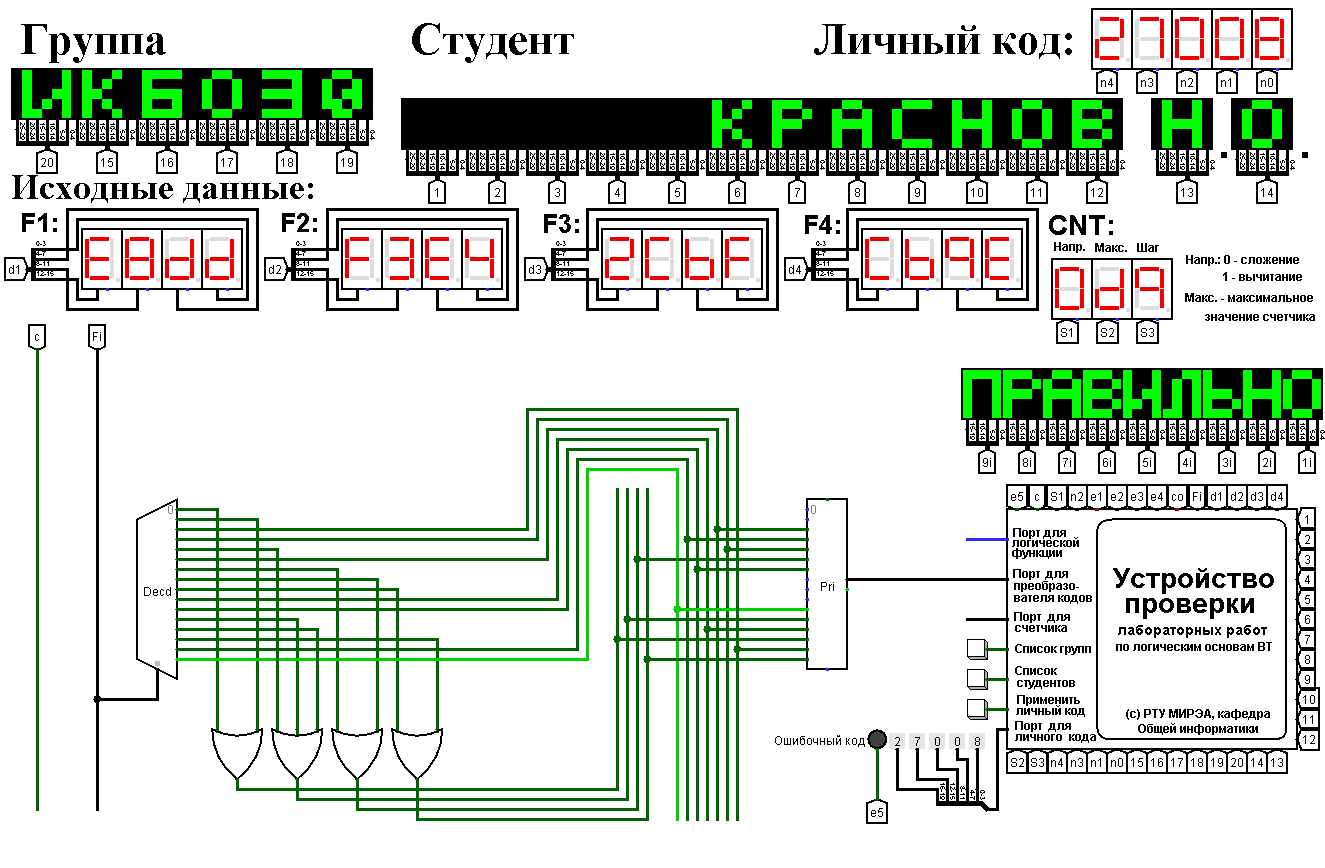
\includegraphics[width=\textwidth]{Преобразователь кодов.png}
	\caption{Схема, реализующая преобразователь кодов}
	\label{fig:Преобразователь}
\end{figure}

\chapter{ВЫВОДЫ}
В ходе работы была восстановлена таблица истинности преобразователя кодов от четырех переменных в реализации дешифратора, шифратора и дополнительной логики <<ИЛИ>>. После реализации работа схемы была протестирована, что позволило убедиться в правильности её работы.

\begin{thebibliography}{99}
	\bibitem{Методичка} \textbf{Смирнов, С. С.} Информатика. Методические указания по выполнению практических работ / С. С. Смирнов, Д. А. Карпов. – Москва, МИРЭА – Российский технологический университет, 2020. – 102 с.
	
	\bibitem{Logisim} \textbf{Берч, К.} / Logisim : среда проектирования логических схем. -- версия 2.7.0. -- [б. м.], 2014. -- URL: http://www.cburch.com/logisim/index.html (дата обращения 26.10.2022). -- Электронная программа : электронная.
\end{thebibliography}

\end{document}
